\documentclass[conference]{IEEEtran}
\IEEEoverridecommandlockouts
% The preceding line is only needed to identify funding in the first footnote. If that is unneeded, please comment it
% out.
\usepackage{cite}
\usepackage{amsmath,amssymb,amsfonts}
\usepackage{algorithmic}
\usepackage{graphicx}
\usepackage{textcomp}
\usepackage{xcolor}
\def\BibTeX{{\rm B\kern-.05em{\sc i\kern-.025em b}\kern-.08em T\kern-.1667em\lower.7ex\hbox{E}\kern-.125emX}}

\usepackage{pdfpages}
\usepackage{steinmetz} % for imaginary numbers
\usepackage[utf8]{inputenc}
\usepackage[english]{babel}
\usepackage[]{amsmath}
\usepackage[]{amssymb}
\usepackage{amsfonts}
\usepackage{hyperref}
\usepackage{graphicx}   % for graphics
\usepackage{xcolor}
\usepackage{float}
\usepackage[font=small,skip=0pt]{caption}
\usepackage{mathtools}
\usepackage{multirow}
\usepackage{multicol}
\usepackage[normalem]{ulem}
\useunder{\uline}{\ul}{}
\DeclarePairedDelimiter{\ceil}{\lceil}{\rceil}

\setcounter{tocdepth}{3}
\setcounter{secnumdepth}{4}

% \setlength{\parindent}{0em} % remove para indents \setlength{\parskip}{1em}

\title{ECE4580 Final Project: \\ Webcam Effects Processor \\\vspace*{20pt}}

\author{\IEEEauthorblockN{Mihir Savadi} mihirsavadi1@vt.edu \\ \today}

% \author{Mihir Savadi \\ }

\begin{document}

    \maketitle
    \IEEEpubid{\today{}\space(\currenttime)}

    % to get page numbers to show up.
    \thispagestyle{plain}
    \pagestyle{plain}

    \begin{abstract}
        For my final project I created a GUI interface and software pipeline for realtime video effects processing. I
        implemented one effect, a cartoonizer, who's algorithm had to be written with an emphasis on execution speed in
        order to maintain a good frame rate. This report briefly explains my efforts.
    \end{abstract}

    % \tableofcontents

    \section{The Problem}

        The goal for this project was to create a software pipeline that would allow a user to both adjust and live
        preview visual effects from a camera feed (ideally their own webcam) in real time. Such an application would
        require the lowest latency possible in effects processing algorithms in order to achieve acceptable frame rates,
        especially given that no complex GPU hardware acceleration schemes were intended to be used. Additionally, in
        order to ensure good code reuse, and effects/feature expandability (both in the front and back end), a well
        designed object orientated software pipeline was required. These were the major challenges in the implementation
        of this project. The repository containing the source code is available at \cite{repo}.

    \section{Approach and Experimental Results}
        
        In order to implement a robust and expandable software pipeline I made use of pythons module import and object
        orientated programming framework. I solely used numpy and OpenCV to implement both the front end and the back
        end, which was possible due to OpenCV having an API for access to its QT underpinnings. The webcam feed was
        handled solely with an OpenCV API call, which abstracted the video feed into iterative frames, which were
        processed in a continuous while loop. 

        For demonstration purposes, I implemented a single effect - a cartoonizer. This involved blurring, edge
        detection, and composition \cite{cartoonification}. I chose to implement gaussian blurring in the frequency
        domain. I had done this before in previous class assignments however with very poor latency (well over 20
        seconds) due to the extensive use of array iteration using for loops. By re-assessing my algorithm and
        converting it to entirely matrix based operations in numpy, as well as employing some other algorithmic
        optimizations, I was able to bring the latency down to 800 milliseconds for the same input webcam frame -- an
        over $25\times$ improvement. Further optimizations are possible such as a one-time pre-computation of
        `distance-from-center' matrices and other constant matrices given a known video feed frame size. The code for
        this can be found here
        \footnote{\url{https://github.com/mihirsavadi/Webcam-EffectsProcessor/blob/master/utils/freqDomain_utils.py}}. A
        similar approach was taken with the implementation of edge-detection, which was done in the spatial domain. The
        code for that can be found here
        \footnote{\url{https://github.com/mihirsavadi/Webcam-EffectsProcessor/blob/master/utils/spatialDomain_utils.py}}.
        Finally the entire cartoonification method can be found here
        \footnote{\url{https://github.com/mihirsavadi/Webcam-EffectsProcessor/blob/master/frame_effects/effects.py}}. It
        should be noted that all of these effects were to be processed on 3-channel color images. Splitting the channels
        and running the effects on each of them before recombining proved to be slow, so 3 dimensional matrix operations
        had to be implemented as opposed to 2 to reduce latency.

        All in all the software pipeline proved to be successful. However due to OpenCV-QT compilation issues some GUI
        features were omitted -- the code for this however is still included in the repository. The cartoonification
        processing worked well, although there is still room for improvement with latency reduction and effects quality.
        Figure~\ref{guiscreenshot} is a screenshot of the application running.
        

        \begin{figure}[H]
            \centering
            \captionsetup{justification=centering}
            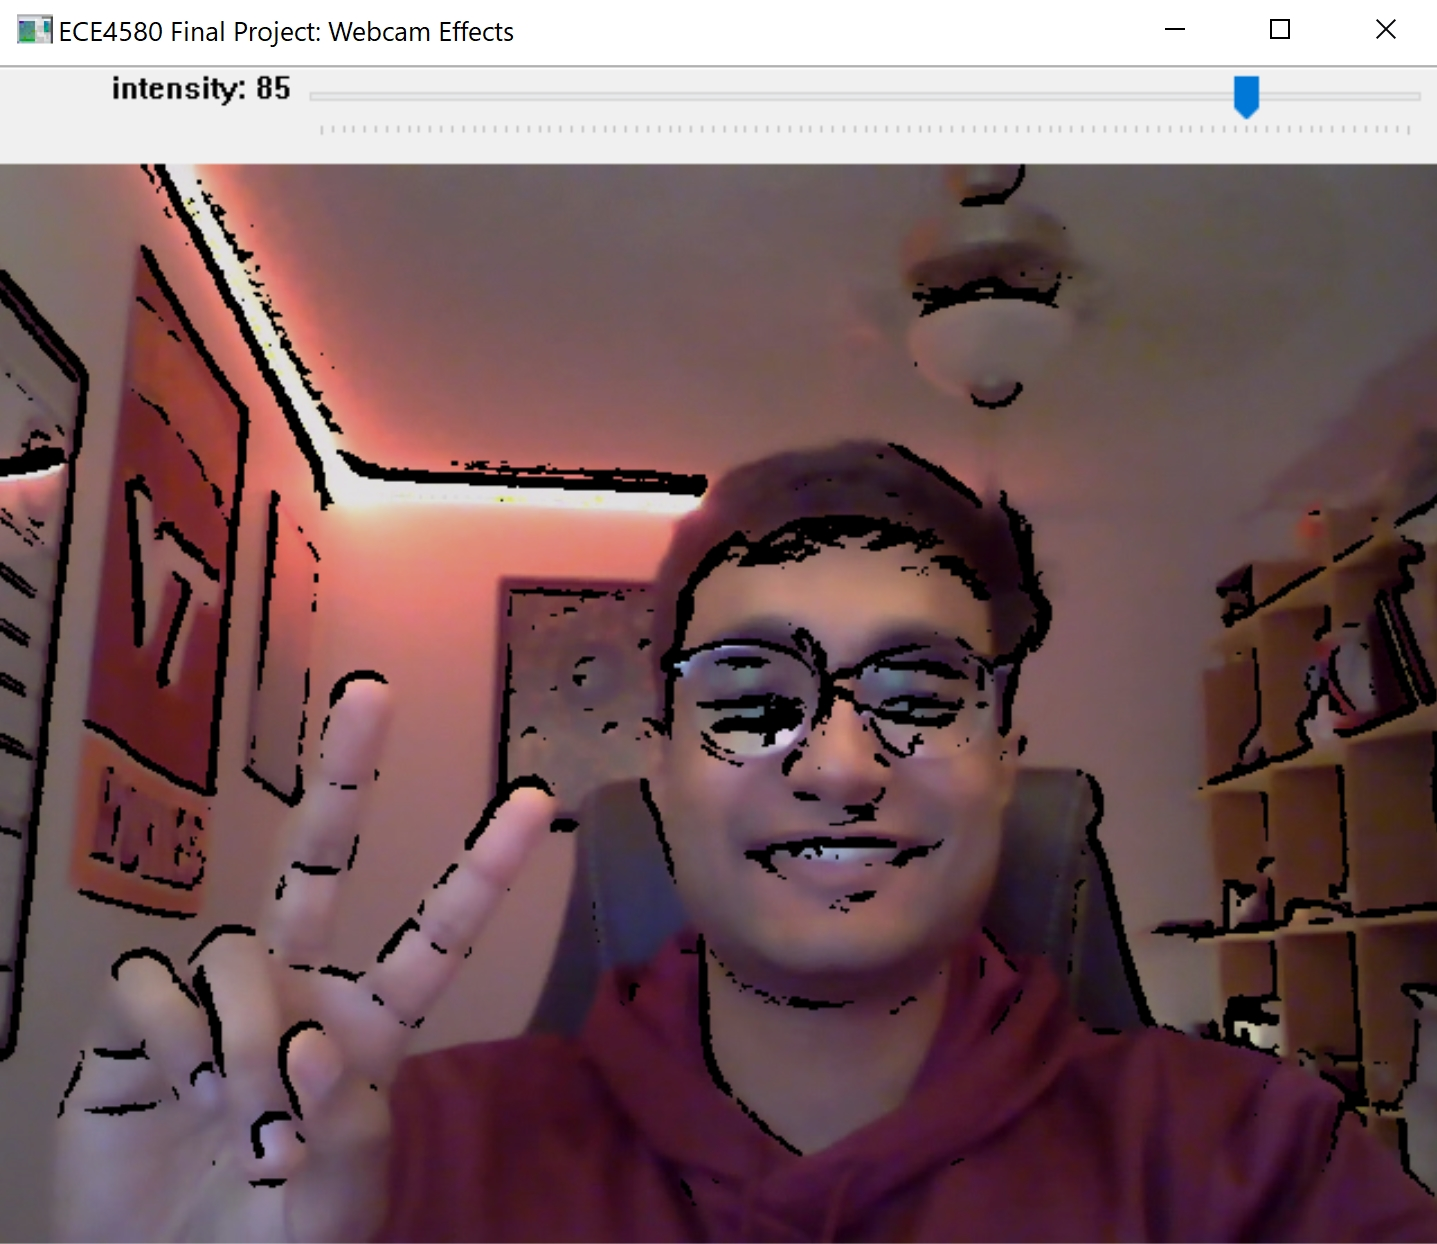
\includegraphics[width=\linewidth]{test/gui_screenshot.jpg}
            \caption{Screenshot of the application running.}
            \label{guiscreenshot}
        \end{figure}


    \begin{thebibliography}{9}

        \bibitem{repo}
            M. Savadi (2021) Webcam-EffectsProcessor [Source Code].
            \url{https://github.com/mihirsavadi/Webcam-EffectsProcessor}
            
        \bibitem{cartoonification}
            data-flair.training (2020) Cartoonify an Image with OpenCV in Python [Article]
            \url{https://data-flair.training/blogs/cartoonify-image-opencv-python/}
        
    \end{thebibliography}

    % \appendices \section{High-level Verification Verilog and Python files, and testbench screenshot}
    % \includepdf[pages=-]{verilog_files/verificationFiles.pdf}
    
\end{document}
